\documentclass[conference]{IEEEtran}
\usepackage{amsmath,amssymb,graphicx,booktabs,cite,url}
\graphicspath{{../plots/}{plots/}}
\def\UrlBreaks{\do\/\do\-\do\.}
\newcommand{\HeldN}{1000}
\newcommand{\HeldInt}{1000}
\newcommand{\HeldFail}{0.38}
\newcommand{\HeldPulses}{9204}
\newcommand{\HeldPulseRate}{99.93}
\newcommand{\HeldFirstMean}{1.24}
\newcommand{\HeldFirstPNN}{1.82}
\newcommand{\HeldFirstMax}{2.35}
\newcommand{\HeldRmsMed}{0.56}
\newcommand{\HeldRmsPNN}{0.83}
\newcommand{\HeldInReng}{99.4}
\newcommand{\HeldVpeak}{589}
\newcommand{\HeldMissMax}{3.35}
\newcommand{\HeldSeedLo}{5000}
\newcommand{\HeldSeedHi}{5999}
\newcommand{\DesWc}{4.10}
\newcommand{\DesPM}{68.5}
\newcommand{\DesGM}{16.1}
\newcommand{\DesMs}{1.21}
\newcommand{\DesKmaxP}{10484}
\newcommand{\DesKmax}{6.35}
\newcommand{\DesKa}{3.99}
\newcommand{\DesKp}{4000}
\newcommand{\DesIlim}{10}
\newcommand{\EbRaw}{0.70}
\newcommand{\EbFilt}{0.42}
\newcommand{\EbBo}{2.52}
\newcommand{\BrierRaw}{0.00285}
\newcommand{\BrierCal}{0.00285}
\newcommand{\AblN}{60}
\newcommand{\AblSeedLo}{201}
\newcommand{\AblSeedHi}{260}
\newcommand{\AimInt}{19}
\newcommand{\AimFirst}{1.22}
\newcommand{\AimRms}{31.09}
\newcommand{\AimPulseRate}{100.0}
\newcommand{\AimMiss}{0}
\newcommand{\AimPulses}{27}
\newcommand{\RobN}{30}
\newcommand{\TimeMean}{0.53}
\newcommand{\TimeMed}{0.52}
\newcommand{\TimePNN}{0.73}
\newcommand{\IndMissWeave}{0}
\newcommand{\IndMissStep}{1}
\newcommand{\IndMissBang}{8}
\newcommand{\IndMissArc}{1}
\newcommand{\IndMissPopup}{3}
\newcommand{\IndConfigs}{6}
\newcommand{\IndCases}{500}
\newcommand{\IndRuns}{3000}
\newcommand{\IndIntMin}{500}
\newcommand{\IndFail}{0.76}
\newcommand{\IndMissCases}{13}
\newcommand{\IndMissLo}{4}
\newcommand{\IndMissHi}{7}
\newcommand{\SwRuns}{54}
\newcommand{\SwHits}{54}
\newcommand{\SwMissN}{2}
\newcommand{\SwFreqA}{100}
\newcommand{\SwMissTA}{1.84}
\newcommand{\SwMissDA}{2.15}
\newcommand{\SwFirstA}{2.85}
\newcommand{\SwThetaA}{80}
\newcommand{\SwFreqB}{1000}
\newcommand{\SwMissTB}{1.85}
\newcommand{\SwMissDB}{2.11}
\newcommand{\SwFirstB}{2.85}
\newcommand{\SwThetaB}{80}
\newcommand{\SaMiss}{2.11}
\newcommand{\SaFilt}{1.24}
\newcommand{\SaSeen}{0.87}
\newcommand{\SaSig}{0.33}
\newcommand{\SaRatio}{3.8}
\newcommand{\SaP}{0.997}
\newcommand{\SaPsure}{0.99}
\newcommand{\SaDrawMin}{0.62}
\newcommand{\SaDrawMax}{1.71}
\newcommand{\SaDrawsOver}{0}
\newcommand{\SaDraws}{10}
\newcommand{\PlJeq}{3200}
\newcommand{\PlA}{320}
\newcommand{\PlB}{3350}
\newcommand{\PlC}{1.0015}
\newcommand{\PlGain}{1000}
\newcommand{\PlPoleRe}{5.23}
\newcommand{\PlPoleIm}{55.70}
\newcommand{\PlWn}{55.9}
\newcommand{\PlHz}{8.90}
\newcommand{\PlZeta}{0.094}
\newcommand{\FfOne}{0.32}
\newcommand{\FfTwo}{3.35}
\newcommand{\FfThree}{1001.5}
\newcommand{\Vlim}{600}
\newcommand{\OmegaCruise}{0.599}
\newcommand{\AcqAccel}{2.5}
\newcommand{\GenPole}{20}
\newcommand{\PiTi}{1}
\newcommand{\PiTauF}{0.03}
\newcommand{\SigJerk}{20}
\newcommand{\TauJerk}{0.4}
\newcommand{\Tp}{0.5}
\newcommand{\PsureV}{0.99}
\newcommand{\ParmV}{0.90}
\newcommand{\PcoastV}{0.95}
\newcommand{\TwaitV}{0.3}
\newcommand{\StepOs}{15.0}
\newcommand{\StepRise}{0.31}
\newcommand{\StepTs}{2.63}
\newcommand{\DesRatio}{13.7}
\newcommand{\PsureAfterV}{0.995}
\newcommand{\SuDFirstLo}{0.70}
\newcommand{\SuDFirstHi}{1.23}
\newcommand{\SuDRmsHi}{0.87}
\newcommand{\SuDInLo}{96}
\newcommand{\SuDAllHit}{every pulse hit}
\newcommand{\ScMaxA}{1.26}
\newcommand{\ScFirstA}{0.94}
\newcommand{\ScPulsesA}{9}
\newcommand{\ScRmsA}{0.40}
\newcommand{\ScMaxB}{1.25}
\newcommand{\ScFirstB}{0.94}
\newcommand{\ScPulsesB}{9}
\newcommand{\ScRmsB}{0.51}
\newcommand{\ScMaxC}{1.08}
\newcommand{\ScFirstC}{0.94}
\newcommand{\ScPulsesC}{9}
\newcommand{\ScRmsC}{0.37}
\newcommand{\EstNowRmsA}{0.25}
\newcommand{\EstNowMaxA}{0.65}
\newcommand{\EstSigA}{0.29}
\newcommand{\EstPredRmsA}{1.33}
\newcommand{\EstPredMaxA}{4.11}
\newcommand{\EstVelRmsA}{1.97}
\newcommand{\EstVelSigA}{3.12}
\newcommand{\EstNowRmsB}{0.32}
\newcommand{\EstNowMaxB}{1.02}
\newcommand{\EstSigB}{0.31}
\newcommand{\EstPredRmsB}{2.16}
\newcommand{\EstPredMaxB}{6.15}
\newcommand{\EstVelRmsB}{3.08}
\newcommand{\EstVelSigB}{3.65}
\newcommand{\EstNowRmsC}{0.26}
\newcommand{\EstNowMaxC}{0.72}
\newcommand{\EstSigC}{0.28}
\newcommand{\EstPredRmsC}{1.07}
\newcommand{\EstPredMaxC}{2.62}
\newcommand{\EstPredBlkC}{2.63}
\newcommand{\EstVelRmsC}{2.06}
\newcommand{\EstVelSigC}{2.94}
\newcommand{\EstBlkSigStart}{0.48}
\newcommand{\EstBlkSigEnd}{2.59}
\newcommand{\EstBlkErrEnd}{0.81}
\newcommand{\EstBlkPredEnd}{2.63}
\newcommand{\FeMin}{0.49}
\newcommand{\FeMedian}{1.24}
\newcommand{\FeLeShare}{71}
\newcommand{\FeRmsMax}{1.31}
\newcommand{\FeRmsOver}{12}
\newcommand{\FeIndLoMean}{1.36}
\newcommand{\FeIndLoPNN}{2.35}
\newcommand{\FeIndLoMax}{3.95}
\newcommand{\FeIndMidMean}{1.07}
\newcommand{\FeIndMidPNN}{1.95}
\newcommand{\FeIndMidMax}{2.51}
\newcommand{\FeIndHiMean}{1.08}
\newcommand{\FeIndHiPNN}{2.00}
\newcommand{\FeIndHiMax}{2.53}
\newcommand{\AblGuardDt}{+0.21}
\newcommand{\AblGuardMiss}{0}
\newcommand{\AblGuardPt}{0.003}
\newcommand{\AblBrakeDt}{+0.11}
\newcommand{\AblBrakeMiss}{2}
\newcommand{\AblBrakePt}{0.003}
\newcommand{\AblPdevTenDt}{+0.50}
\newcommand{\AblPdevTenMiss}{0}
\newcommand{\AblPdevTenPt}{0.003}
\newcommand{\AblRateDt}{+0.35}
\newcommand{\AblRateMiss}{1}
\newcommand{\AblRatePt}{0.003}
\newcommand{\AblLeadDt}{-0.00}
\newcommand{\AblLeadMiss}{0}
\newcommand{\AblLeadPt}{1.000}
\newcommand{\AblNoAdaptDt}{-0.00}
\newcommand{\AblNoAdaptMiss}{0}
\newcommand{\AblNoAdaptPt}{1.000}
\newcommand{\AblNoFreezeDt}{-0.01}
\newcommand{\AblNoFreezeMiss}{0}
\newcommand{\AblNoFreezePt}{1.000}
\newcommand{\RobRefRms}{0.56}
\newcommand{\RobRefFirst}{1.20}
\newcommand{\RobLowRateRms}{0.99}
\newcommand{\RobLowRateFirst}{1.47}
\newcommand{\RobKtKeRms}{3.74}
\newcommand{\RobKtKeFirst}{1.82}
\newcommand{\RobAllInt}{690}
\newcommand{\RobAllN}{690}
\newcommand{\RobRows}{23}
\newcommand{\LosRelOneM}{9.8\times10^{-4}}
\newcommand{\LosSlope}{2}
\newcommand{\LosRawLo}{0.28}
\newcommand{\LosRawHi}{0.70}
\newcommand{\LosUseLo}{14}
\newcommand{\LosUseHi}{35}
\newcommand{\LosBlkLo}{1.70}
\newcommand{\LosBlkHi}{2.52}
\newcommand{\LosBlkCross}{1200}
\newcommand{\SensMt}{1.17}
\newcommand{\SensWb}{5.72}
\newcommand{\SensEncT}{0.15}
\newcommand{\SensTNyq}{-21.4}
\newcommand{\SensWMs}{52}
\newcommand{\SensWs}{2.8}
\newcommand{\SpecZetaOne}{1.04}
\newcommand{\SpecWnOne}{2.16}
\newcommand{\SpecReqOs}{20}
\newcommand{\SpecEThreeMax}{4}
\newcommand{\SpecReqTr}{0.5}
\newcommand{\SpecReqTs}{3}
\newcommand{\UncPMmin}{67.1}
\newcommand{\UncGMmin}{10.7}
\newcommand{\UncKmin}{3.42}
\newcommand{\CompKvP}{3.99}
\newcommand{\CompPmP}{89}
\newcommand{\CompGmP}{8.4}
\newcommand{\CompGmPhi}{2.3}
\newcommand{\CompPhiNeeded}{-18.4}
\newcommand{\CompGmLeadLo}{5.0}
\newcommand{\CompGmLeadHi}{-5.7}
\newcommand{\CompRampM}{38}
\newcommand{\CompNoiseRatio}{4.0}
\newcommand{\CompKvLim}{10.5}
\newcommand{\DelayMargin}{0.29}
\newcommand{\DelayPMZoh}{62.6}
\newcommand{\DelayPMLat}{56.7}
\newcommand{\DelayHold}{75}
\newcommand{\DelayCoast}{6.0}
\newcommand{\DelaySafeFive}{14.1}
\newcommand{\DelaySafeHund}{4.1}
\newcommand{\DelayWbHund}{5.7}
\newcommand{\DelayDegTen}{2.4}
\newcommand{\DelayTdFortyFive}{0.10}
\newcommand{\SampWeq}{0.32}
\newcommand{\SampNyq}{62.8}
\newcommand{\SampResPct}{89}
\newcommand{\SampZohDeg}{5.9}
\newcommand{\SampPerSample}{7.5}
\newcommand{\SampPMTwenty}{62.6}
\newcommand{\SampGMTwenty}{17.6}

\newcommand{\teamauthors}{Shourya Saxena (24b2222), Shashwat Gupta (24b2237),\\ Surhud Naik (24b2111), Jay Motwani (24b2172)}
\begin{document}
\title{Predictive Tracking and Turret Control for a Maneuvering Aerial Target:\\ a Nowcast-Referenced Two-Degree-of-Freedom Design}
\author{\IEEEauthorblockN{\teamauthors}\IEEEauthorblockA{ME 319 Control Systems, Autumn 2026, IIT Bombay\\ Code: \url{https://github.com/Charon-68/Turrent-Control-System_ME319/tree/master}}}
\maketitle

\begin{abstract}
A pulsed laser turret must hit a maneuvering drone from noisy 20~Hz radar, through blackouts of up to 0.5~s, using a lightly damped elevation drive. The design combines a converted-measurement Kalman filter with a Markov-jerk target model, exact line-of-sight derivatives, a reference generator that cancels the prescribed \Tp~s Taylor advance, an exact-inverse feed-forward with a PI loop (phase margin \DesPM$^\circ$, gain margin \DesGM~dB), and a fire rule on a posterior hit probability. The single frozen design was evaluated on \HeldN{} held-out random engagements (\HeldInt/\HeldN{} intercepted, Wilson 95\,\% failure bound $<\HeldFail\,\%$, mean first hit \HeldFirstMean~s), on \IndRuns{} runs of an independent generator written by the project team (\IndIntMin/\IndCases{} intercepted in every configuration), and on interface variants covering call rate, flag convention, start angle and plant mismatch. Margin studies quantify the operating envelope: the first pulse from an $80^\circ$ start lands \SaMiss~m from the target, and the pointing RMS is \RobKtKeRms~m when $K_t$ and $K_e$ are both 20\,\% off. The architecture was build from scratch using multiple research paper implementations as mentioned in the references.
\end{abstract}

\section{Introduction}
The elevation axis of a laser turret must point at a maneuvering target seen only through a 20~Hz radar (range noise $\sigma_r=1$~m, bearing noise $\sigma_\theta=0.02^\circ$) that may go blind for up to 0.5~s from 1~s on. A pulse hits if the beam passes within $R_{eng}=2$~m of the target; pulses are at least 1~s apart. The objectives are interception (a hit within $0\le t\le10$~s), early interception (the first hit sets the interception time) and accurate, consistent pointing, with one frozen estimator, predictor and linear time-invariant (LTI) compensator for all cases.

The handout leaves several quantities open; the design adopts the following assumptions (consequences in \texttt{docs/ASSUMPTIONS.md}): a supply limit $|V_m|\le\Vlim$~V, a motor-current budget of \DesIlim~A (it bounds only the acquisition acceleration), an initial turret angle of 0 unless stated, the initial conditions and maneuver shapes of scenarios A--C, and an evaluator that integrates the plant with steps of at most 1~ms and judges pulses at its call instants.

The filter is a Kalman filter~\cite{kalman} on converted Cartesian measurements~\cite{barshalom,lerro} with a Gauss--Markov target model~\cite{mehrotra}, in the spirit of the correlated-acceleration model of Singer~\cite{singer} one derivative higher (jerk); the loop is analysed with the course methods~\cite{lecture}. The architecture (converted-measurement filter with a Markov-jerk model, exact line-of-sight derivatives, a reference generator that cancels the prescribed $t_p$ advance, exact-inverse feed-forward plus PI feedback, a hit-probability fire rule) builds from a research paper. Here it is re-implemented in GNU Octave with every gain and clamp derived from one parameter file, and extended with closed-form transition matrices, a posterior hit probability, adaptive process noise, a stop governor, a held-out seed protocol and an independent check.

\section{System Architecture and Design}
Fig.~\ref{fig:geom} shows the geometry and Fig.~\ref{fig:loop} the information flow. The Kalman filter turns the radar samples $(r,\theta)$ into a target state (position, velocity, acceleration, jerk per axis), propagated to the present call time (nowcast). The elevation angle and its first three derivatives $D=(\hat\theta,\hat\theta',\hat\theta'',\hat\theta''')$ follow exactly from it, and the Taylor prediction of the elevation $t_p=\Tp$~s ahead is a fixed linear combination of $D$ (Section~\ref{sec:pred}). A reference generator turns it into a smooth reference $y_d$ with three derivatives, from which an exact plant inverse (feed-forward) and a PI loop produce the voltage $V_m$. In parallel, the estimator state feeds a hit probability and a fire-now-or-wait rule that issues \texttt{fire\_cmd}.
\begin{figure}[t]\centering
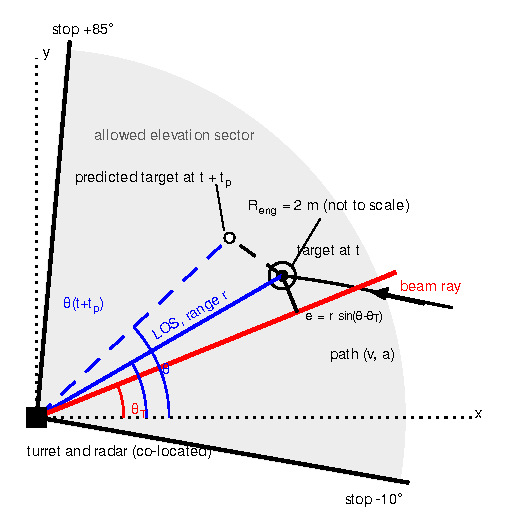
\includegraphics[width=\columnwidth]{report_schematic.pdf}
\caption{Elevation-plane geometry. The turret and radar are co-located; the beam is a ray along $\theta_T$; a hit needs $|e|\le R_{eng}$. The $R_{eng}$ ring and the $t_p$ advance are drawn exaggerated.}\label{fig:geom}
\end{figure}
\begin{figure*}[t]\centering
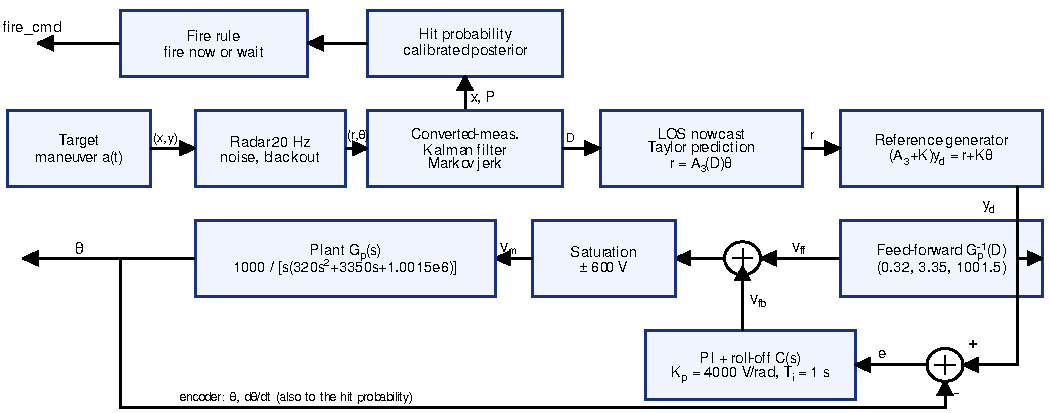
\includegraphics[width=0.97\textwidth]{report_blockdiagram.pdf}
\caption{Closed-loop block diagram of the predictive-feedback design. Numbers are read from the parameter file.}\label{fig:loop}
\end{figure*}

\section{Mathematical Modeling}
\subsection{Plant}
With armature current $i$, turret angle $\theta_T$, motor voltage $V_m$, $R=1~\Omega$ and $L=0.1$~H,
\begin{equation}
L\dot i=V_m-Ri-NK_e\dot\theta_T,\qquad J_{eq}\ddot\theta_T=NK_ti-b\dot\theta_T,
\end{equation}
with gear ratio $N=100$ (the motor turns $N$ times faster), $K_t=10$~N\,m/A, $K_e=10$~V\,s/rad, $b=1500$~N\,m\,s/rad and reflected inertia $J_{eq}=J_t+N^2J_m=\PlJeq$~kg\,m$^2$ ($J_t=1200$, $J_m=0.20$~kg\,m$^2$). Eliminating $i$,
\begin{equation}
\begin{split}
G_p(s)&=\frac{NK_t}{s\left[(Ls+R)(J_{eq}s+b)+N^2K_tK_e\right]}\\
&=\frac{\PlGain}{s(\PlA s^2+\PlB s+\PlC{\cdot}10^{6})}.
\end{split}
\end{equation}
The pole at the origin integrates rate to angle; the pair $-\PlPoleRe\pm j\PlPoleIm$~rad/s (\PlWn~rad/s, \PlHz~Hz, $\zeta=\PlZeta$) is the lightly damped electromechanical mode; the relative degree is three. The model is the linearised small-perturbation plant, valid inside the stops $-10^\circ\le\theta_T\le85^\circ$ and for $|V_m|\le\Vlim$~V, with viscous damping only (Coulomb friction and a dead zone are variants in Section~\ref{sec:fe}).

\subsection{Target and measurement model (estimation)}
Each Cartesian axis carries $\mathbf x=(p,v,a,j)^\top$ with $\dot p=v$, $\dot v=a$, $\dot a=j$ and $\dot j=-j/\tau_j+w$ (the jerk model of~\cite{mehrotra}), $w$ white with intensity set by $\sigma_j=\SigJerk$~m/s$^3$ and $\tau_j=\TauJerk$~s. The transition $F(\tau)$ and noise $Q(\tau)$ for any gap $\tau$ are computed in closed form, so a blackout is a long gap: the filter propagates and its covariance grows. The measurement is converted to $(x,y)=(r\cos\theta,r\sin\theta)$ with the unbiased correction and its exact covariance~\cite{barshalom,lerro}, which keeps the update linear. A $\chi^2$ gate rejects implausible innovations, estimates are projected onto the speed and acceleration envelope, the process noise is scaled by a normalised-innovation statistic, and repeated samples are ignored, so either \texttt{meas\_valid} convention works.

\subsection{Prediction and elevation reference}\label{sec:pred}
With $z=x+jy$ and $w_k=z^{(k)}/z$ the elevation and its derivatives follow exactly from the nowcast, $\theta'=\mathrm{Im}\,w_1$, $\theta''=\mathrm{Im}(w_2-w_1^2)$, $\theta'''=\mathrm{Im}(w_3-3w_1w_2+2w_1^3)$. The Taylor prediction of the elevation $t_p$ ahead is
\begin{equation}
r=A_3(D)\hat\theta,\qquad A_3(s)=1+t_ps+\tfrac12(t_ps)^2+\tfrac16(t_ps)^3,
\end{equation}
with $D=d/dt$. The laser is instantaneous, so a hit needs the beam on the \emph{present} bearing; aiming at $r$ would miss by about $r_\mathrm{LOS}\dot\theta t_p$, tens of metres. The prediction is therefore not the pointing target but the input of a reference generator $(A_3+K)(D)\,y_d=r+K(D)\hat\theta$ with $A_3+K=\tfrac{t_p^3}{6}(s+p)^3$, $p=\GenPole$~rad/s. Substituting $r$,
\begin{equation}
(D+p)^3\,(y_d-\hat\theta)=0,
\end{equation}
so $y_d$ follows the nowcast through a triple pole, $y_d,\dot y_d,\ddot y_d,\dddot y_d$ are available without differentiating noise, and the loop does not depend on $t_p$. Aiming at the predicted bearing instead intercepted only \AimInt{} of \AblN{} paired engagements (Section~\ref{sec:fe}).

\subsection{Closed-loop model used for design}\label{sec:loopmodel}
The voltage is $V_m=G_p^{-1}(D)\,y_d+C(s)\,(y_d-\theta_T)$, clipped to $\pm\Vlim$~V, with
\begin{equation}
\begin{split}
C(s)&=K_p\frac{T_is+1}{T_is(\tau_fs+1)},\\
K_p&=\DesKp~\mathrm{V/rad},\ T_i=\PiTi~\mathrm{s},\ \tau_f=\PiTauF~\mathrm{s}.
\end{split}
\end{equation}
The inverse $G_p^{-1}(D)=\FfOne D^3+\FfTwo D^2+\FfThree D$ is realisable because $y_d$ supplies three derivatives; for the exact plant the feed-forward alone gives $\theta_T=y_d$ and the loop handles model error. The design model is $L=CG_p$, $T=L/(1+L)$, $S=1/(1+L)$.

\section{Controller Design and Analysis}
\subsection{Stability and margins}
For proportional control the characteristic polynomial is $a_2s^3+a_1s^2+a_0s+kNK_t$ with $(a_2,a_1,a_0)=(\PlA,\PlB,\PlC{\cdot}10^6)$; the Routh array gives stability if and only if
\begin{equation}
k<\frac{a_1a_0}{a_2NK_t}=\DesKmaxP~\mathrm{V/rad},
\end{equation}
so $K_p=\DesKp$ is well inside. With the PI term and roll-off the loop is stable up to \DesKmax{} times the design gain (root locus, Fig.~\ref{fig:design}). The crossover is \DesWc~rad/s, \DesRatio{} times below the \PlWn~rad/s resonance, with phase margin \DesPM$^\circ$, gain margin \DesGM~dB and peak sensitivity $M_s=\DesMs$; the resonance is gain-stabilised and needs no notch.
\begin{figure}[t]\centering
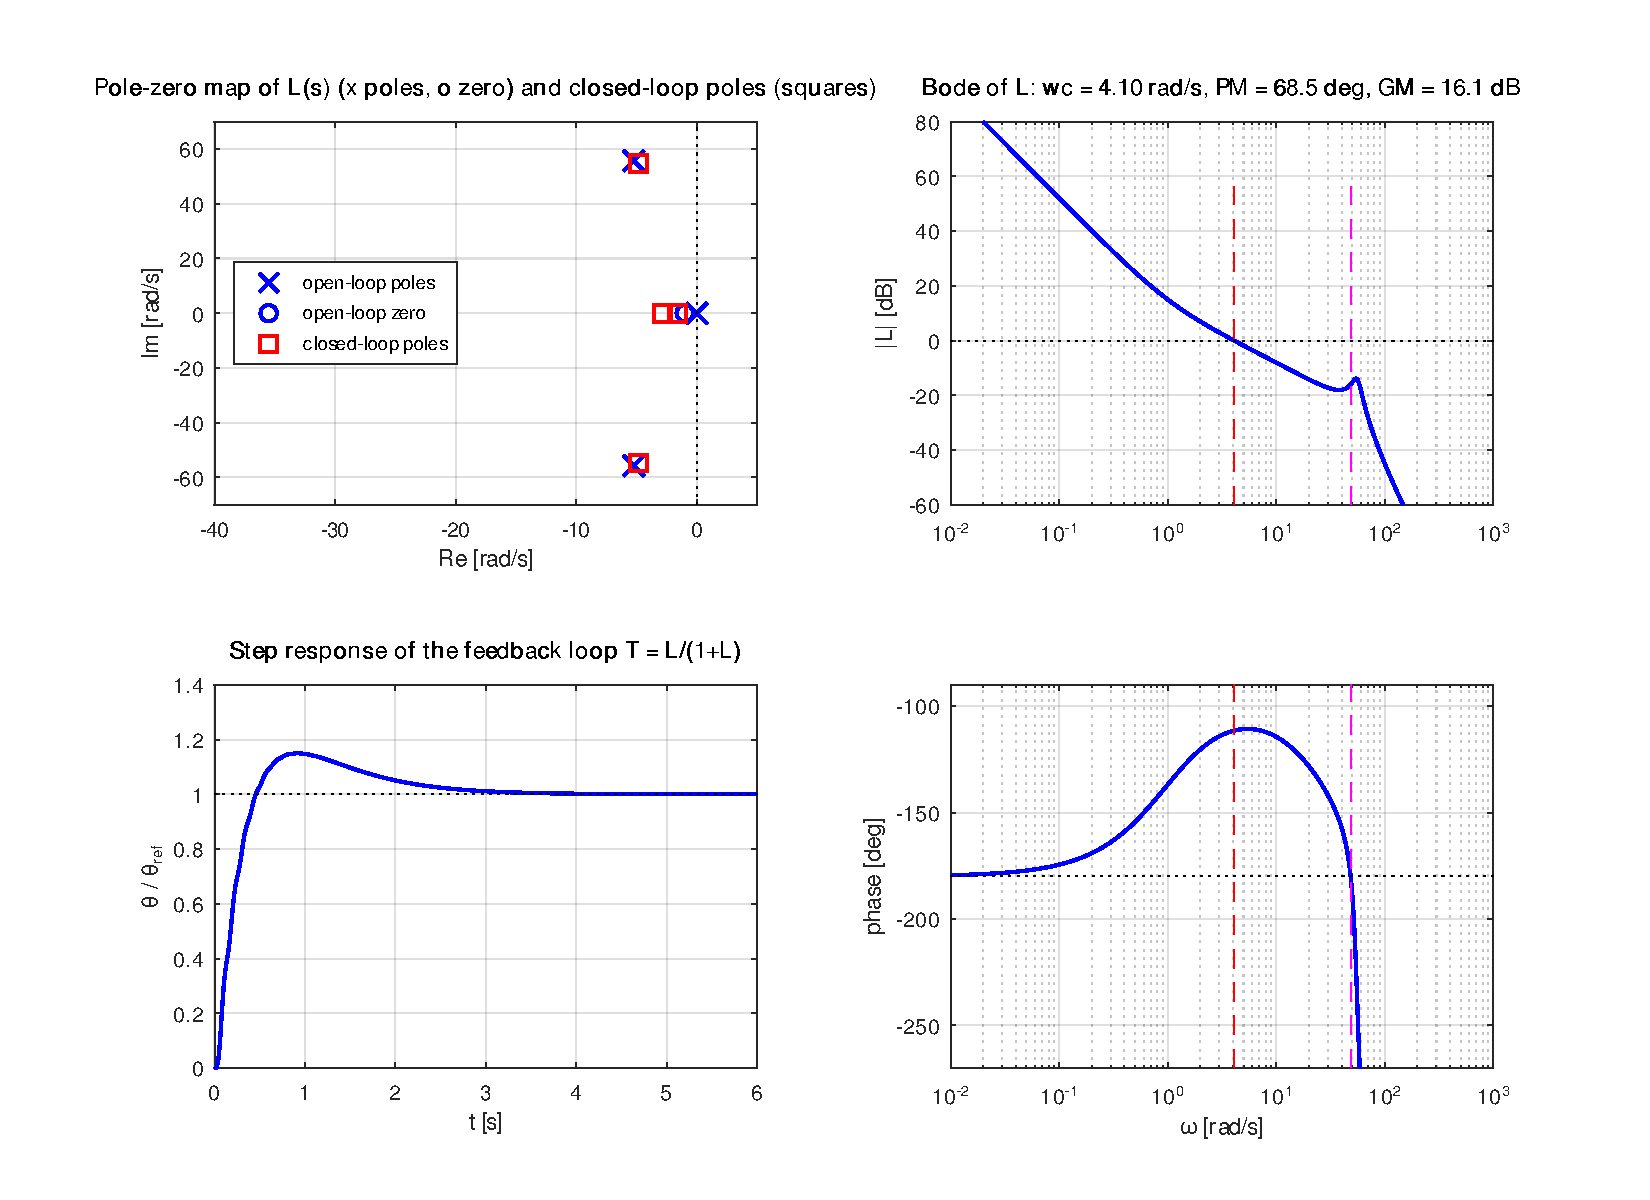
\includegraphics[width=\columnwidth]{design_analysis.pdf}
\caption{Pole-zero map of $L$, Bode plot with margins, and step response of the feedback loop alone.}\label{fig:design}
\end{figure}

\subsection{Steady state, transient response and the lead compensator}\label{sec:ss}
$L$ has two poles at the origin (type two), so by the final value theorem the position and ramp errors vanish and a parabola of angular acceleration $\ddot\theta$ leaves $e_{ss}=\ddot\theta/K_a$ with $K_a=\lim_{s\to0}s^2L(s)=\DesKa$~s$^{-2}$ (an exact partial-fraction simulation reproduces it); the feed-forward removes it for an exact model. The step of $T$ (feedback alone) has overshoot \StepOs\,\%, 10--90\,\% rise \StepRise~s and 2\,\% settling \StepTs~s, against self-set targets (the handout prescribes none: ($\le\SpecReqOs\,\%$, $\le\SpecReqTr$~s, $\le\SpecReqTs$~s)). The two slowest poles are real ($\zeta=\SpecZetaOne$) and near the PI zero, so no dominant pair exists: the two-pole estimate shows no overshoot at all, and adding the zero reproduces the response within \SpecEThreeMax\,\% (\texttt{outputs/tc\_study\_specs.txt}). The lecture lead-compensator procedure asks for a phase lead of $\CompPhiNeeded^\circ$, that is, none; a proportional loop has PM \CompPmP$^\circ$ but is type one (ramp error about \CompRampM~m at the worst LOS rate), and a forced lead of $30^\circ$ lowers the gain margin to \CompGmLeadHi--\CompGmLeadLo~dB, so the PI with roll-off is kept.
\subsection{Noise, delay, sampling and parameter error}
Radar noise reaches the turret through $T$ and the generator: $|T|$ is $\SensTNyq$~dB at the 20~Hz Nyquist frequency, but the noise is flat to Nyquist while the maneuver band lies below \SampWeq~rad/s, so in-band noise is removed by the estimator, not the loop. A delay $T_d$ costs $\omega_cT_d$ of phase margin (\DelayDegTen$^\circ$ per 10~ms): the 20~Hz zero-order hold leaves \DelayPMZoh$^\circ$ and the margin vanishes at \DelayMargin~s. The Nyquist frequency (\SampNyq~rad/s) is far above the LOS content, so nothing aliases. For $\pm20\,\%$ errors in $K_t,K_e,J,b$, including all 16 corners, the linear loop stays stable with PM $\ge\UncPMmin^\circ$ and GM $\ge\UncGMmin$~dB; $K_e$ matters most.

\subsection{Estimation and prediction error, and measurement loss}\label{sec:est}
Fig.~\ref{fig:est} compares the estimator with the true target for scenarios A--C. The nowcast cross-range error has RMS \EstNowRmsA, \EstNowRmsB{} and \EstNowRmsC~m (A, B, C; outside blackouts, $t\ge2$~s), close to the filter's mean $1\sigma$ of \EstSigA, \EstSigB{} and \EstSigC~m; the velocity error RMS is \EstVelRmsA, \EstVelRmsB{} and \EstVelRmsC~m/s against mean $1\sigma$ values of \EstVelSigA, \EstVelSigB{} and \EstVelSigC~m/s. The $t_p$-ahead prediction error is larger, RMS \EstPredRmsA, \EstPredRmsB{} and \EstPredRmsC~m with peaks of \EstPredMaxA, \EstPredMaxB{} and \EstPredMaxC~m, often above $R_{eng}$. In the blackout of scenario C the filter coasts on its model: the nowcast $1\sigma$ grows from \EstBlkSigStart{} to \EstBlkSigEnd~m in 0.5~s (more than $R_{eng}$), the actual nowcast error reaches \EstBlkErrEnd~m and the prediction error \EstBlkPredEnd~m, so the coasting fire rule asks for a higher hit probability before a late shot after a long loss (Section~\ref{sec:fire}).
\begin{figure*}[t]\centering
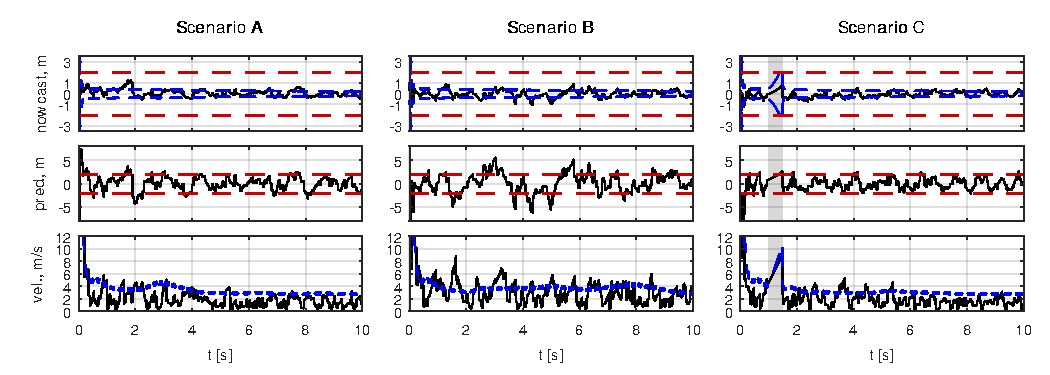
\includegraphics[width=0.97\textwidth]{report_estimation.pdf}
\caption{Estimation and prediction error for scenarios A, B, C (100~Hz): cross-range error of the nowcast (black) with the filter's $\pm1\sigma$ (blue dashed), error of the $t_p$-ahead prediction, and velocity error with its $1\sigma$; red dashed lines mark $\pm R_{eng}$, gray bands the blackout.}\label{fig:est}
\end{figure*}

\section{Fire Control}\label{sec:fire}
The offset between beam and target is Gaussian given the target's acceleration; integrating over the acceleration posterior (truncated to the envelope, 25-node Gauss--Hermite rule) gives the hit probability $P$. While tracking, the rule fires at $P\ge\PsureV$, or arms at $P\ge\ParmV$ and fires when $P$ peaks or after \TwaitV~s; while coasting it fires only if $P\ge\PcoastV$ and falling; after the first pulse the bar is \PsureAfterV. An isotonic calibration of $P$ gave the same held-out Brier score (\BrierRaw) as the identity map, so the raw $P$ is used.

\section{Simulation and Results}
Scenarios A--C follow the handout with our initial conditions and maneuver shapes (A: constant velocity; B: smooth bounded acceleration in $x$ and $y$ from 1~s; C: A with a 0.5~s blackout from 1~s); D1--D6 are additional stress cases. All runs use the frozen design, a 100~Hz controller and a turret starting at $0^\circ$. Additional design parameters are the assumed $\pm\Vlim$~V and \DesIlim~A (the budget sets the acquisition acceleration clamp, \AcqAccel~rad/s$^2$; the rate clamp is 97\,\% of the cruise rate \OmegaCruise~rad/s), the generator pole $p=\GenPole$~rad/s, and the PI, estimator and fire-rule constants above; the PI gains are kept from the reference and re-verified analytically.

Fig.~\ref{fig:scn} shows the three scenarios. The first hit is at \ScFirstA, \ScFirstB{} and \ScFirstC~s (A, B, C), when the initial slew from $0^\circ$ ends, with the voltage on its rate-limited plateau; afterwards the beam error stays below \ScMaxA, \ScMaxB{} and \ScMaxC~m, every pulse hits (\ScPulsesA, \ScPulsesB{} and \ScPulsesC{} pulses), and the pointing RMS is \ScRmsA, \ScRmsB{} and \ScRmsC~m. Scenario B has the largest RMS and also the largest estimation and prediction errors (Fig.~\ref{fig:est}). No pulse falls inside the blackout of C (the first pulse precedes it and the recharge blocks the next), so C tests the filter and loop through a loss but not the coasting fire rule; the held-out family (one blackout per engagement, onset 1--8.5~s, 0.1--0.5~s long) and D1, D4, D5 do. In D1--D6 the first hit is between \SuDFirstLo{} and \SuDFirstHi~s, \SuDAllHit, with pointing RMS at most \SuDRmsHi~m.
\begin{figure*}[t]\centering
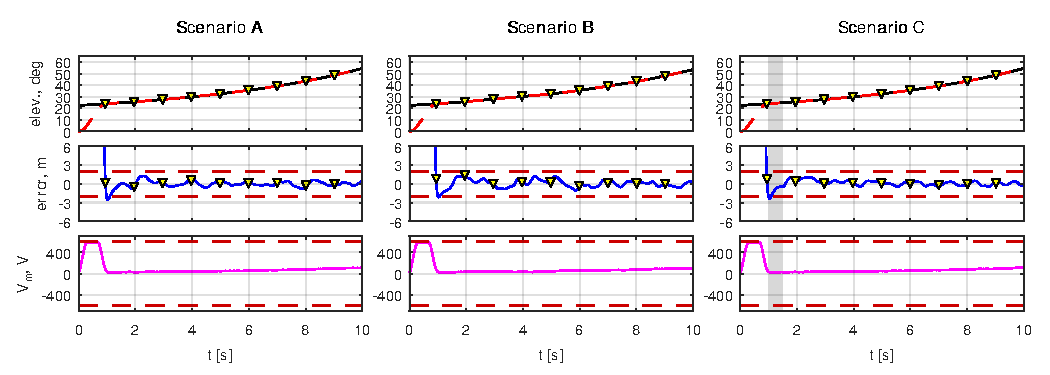
\includegraphics[width=0.97\textwidth]{report_scenarios.pdf}
\caption{Scenarios A, B, C at 100~Hz: target (black) and turret (red dashed) elevation, cross-range beam error with pulses (triangles; filled: hit), and motor voltage; the blackout of C is shaded.}\label{fig:scn}
\end{figure*}

\section{Final Evaluation}\label{sec:fe}
\textbf{Basis.} The finalized design was evaluated on (i) \HeldN{} held-out random engagements from this project's generator, (ii) an independent generator written separately in code but by the same project, and (iii) interface variants (call rates, flag conventions, start angles, plant mismatch). The assumptions of Section~I apply: calls at a multiple of 20~Hz, plant integrated with steps of at most 1~ms, pulses judged at the call instants (\texttt{tests/eval\_adapter.m}).

\textbf{(i) Held-out campaign.} Seeds \HeldSeedLo--\HeldSeedHi{} were never used to choose or fit anything (100~Hz, start $0^\circ$). \HeldInt{} of \HeldN{} intercepted (Wilson 95\,\% failure bound $<\HeldFail\,\%$). The interception time has mean \HeldFirstMean~s, median \FeMedian~s, 95th percentile \HeldFirstPNN~s and maximum \HeldFirstMax~s, set by the initial slew. Of \HeldPulses{} pulses, \HeldPulseRate\,\% were on target (worst miss \HeldMissMax~m). Pointing RMS per run has median \HeldRmsMed~m and 95th percentile \HeldRmsPNN~m (maximum \FeRmsMax~m; above 1~m in \FeRmsOver{} runs); the beam stayed within $R_{eng}$ \HeldInReng\,\% of the time (Fig.~\ref{fig:fe}a,b).

\textbf{(ii) Independent check.} Five families (weave, jerk-limited step, bang-bang, maximum-acceleration arc, pop-up; \IndCases{} cases per configuration, random start, one blackout, random initial turret angle) with their own closed-loop runner were written from the assignment text without reading the scenario library, but by the same project; the check guards against our blind spots and is not an external test. In \IndConfigs{} configurations (20, 100, 1000~Hz; new-sample or held flag) all \IndRuns{} runs intercepted (\IndIntMin/\IndCases{} per configuration, failure bound $<\IndFail\,\%$). Mean first hit is \FeIndLoMean, \FeIndMidMean{} and \FeIndHiMean~s at 20, 100 and 1000~Hz (95th percentile \FeIndLoPNN, \FeIndMidPNN, \FeIndHiPNN~s; maximum \FeIndLoMax, \FeIndMidMax, \FeIndHiMax~s; Fig.~\ref{fig:fe}c). In \IndMissCases{} of \IndCases{} cases a pulse missed (bang-bang \IndMissBang, pop-up \IndMissPopup, step \IndMissStep, arc \IndMissArc, weave \IndMissWeave); the flag conventions give identical rows because the filter discards exact repeats.
\begin{figure*}[t]\centering
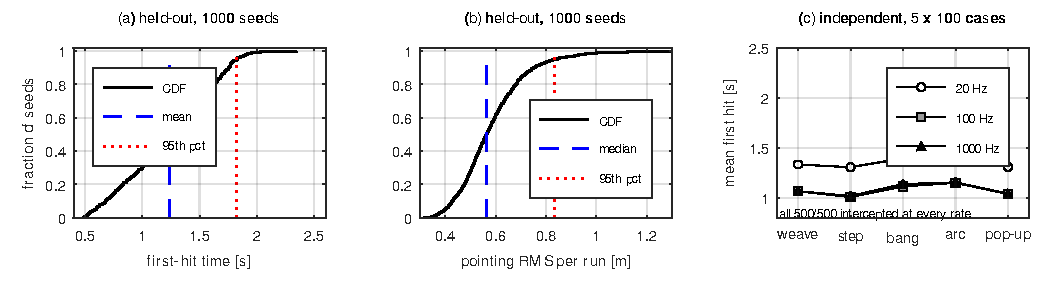
\includegraphics[width=0.97\textwidth]{report_final_eval.pdf}
\caption{Final evaluation. (a) CDF of the first-hit time and (b) of the pointing RMS over the \HeldN{} held-out seeds; (c) mean first-hit time per family of the independent campaign at three call rates.}\label{fig:fe}
\end{figure*}

\textbf{(iii) Interface variants.} Table~\ref{tab:rob} (\RobN{} held-out seeds per row; \RobRows{} rows run, selected rows shown) covers call rate, measurement conventions, start angle, plant mismatch with and without adaptive feed-forward, friction and out-of-spec sensors; all \RobAllInt{} of \RobAllN{} engagements intercepted. The reference row has pointing RMS \RobRefRms~m and mean first hit \RobRefFirst~s; at 20~Hz, \RobLowRateRms~m and \RobLowRateFirst~s. Paired ablations on \AblN{} seeds (\AblSeedLo--\AblSeedHi{}) show no meaningful first-hit change without adaptive process noise, the acquisition freeze or the lead (\AblNoAdaptDt, \AblNoFreezeDt{}, \AblLeadDt~s) and slower first hits with a slip guard (\AblGuardDt~s), a braking-curve slew (\AblBrakeDt~s, \AblBrakeMiss{} missed pulses) or a slower generator pole (\AblPdevTenDt~s).
\begin{table}[t]\centering\caption{Robustness of the frozen design (selected rows of \texttt{outputs/robustness.txt}).}\label{tab:rob}\scriptsize
\begin{tabular}{lrrrr}\toprule
Condition & icpt & miss & $t_1$ [s] & RMS [m]\\\midrule
reference 100 Hz & 30/30 & 0 & 1.20 & 0.56 \\
rate 20 Hz & 30/30 & 1 & 1.47 & 0.99 \\
rate 1 kHz & 30/30 & 0 & 1.20 & 0.53 \\
held last sample & 30/30 & 0 & 1.20 & 0.56 \\
irregular call times & 30/30 & 1 & 1.24 & 0.74 \\
start at -10 deg & 30/30 & 2 & 1.51 & 0.62 \\
Kt +20 \%, Ke -20 \% & 30/30 & 0 & 1.29 & 1.57 \\
Kt -20 \%, Ke +20 \% & 30/30 & 0 & 1.82 & 3.74 \\
  same, adaptive FF & 30/30 & 0 & 1.82 & 3.79 \\
Coulomb 300 Nm + 20 V dead-zone & 30/30 & 0 & 1.20 & 0.72 \\
HB adversarial family & 30/30 & 2 & 1.28 & 0.74 \\
MC + glint (out of spec) & 30/30 & 2 & 1.25 & 0.62 \\
\crcr\bottomrule\end{tabular}\end{table}

\textbf{Operating margins.} \emph{Start at $80^\circ$.} The handout-rule adapter ran \SwRuns{} cases (start angles $0$, $0.3$~rad, $80^\circ$; 20, 100, 1000~Hz); every case reached a hit, and \SwMissN{} pulses landed outside $R_{eng}$: in scenario A from $\SwThetaA^\circ$ the first pulse at 100 and 1000~Hz landed \SwMissDA{} and \SwMissDB{}~m from the target (limit $R_{eng}=2$~m), so the first hit came at \SwFirstA{}~s. A replay of the 100~Hz case traces this to a \SaFilt{}~m filter bearing error plus a \SaSeen{}~m offset seen by the controller, with the hit probability (\SaP{}) above the firing threshold (\SaPsure{}) while the posterior sigma (\SaSig{}~m) was below the real error. The $85^\circ$ stop and the voltage and current limits were ruled out as causes; \SaDrawsOver{} of \SaDraws{} other noise draws exceeded 2~m, so the offset is tied to this particular noise realisation at a large initial slew.
\emph{Parameter sensitivity and other margins.} Pulse misses concentrate in the bang-bang family, the most aggressive maneuver. Accuracy is most sensitive to $K_t$ and $K_e$ errors of 20\,\% in opposite directions (RMS \RobKtKeRms~m, first hit \RobKtKeFirst~s), because the velocity feed-forward is dominated by $NK_e$; the adaptive feed-forward gave no further gain, so the PI loop carries the model error. After a long blackout the nowcast $1\sigma$ exceeds $R_{eng}$ (Section~\ref{sec:est}), which the stricter coasting fire rule accounts for. The $\pm\Vlim$~V and \DesIlim~A values are design assumptions, and the current budget is exceeded only in some mismatch rows. The held-out family is random-admissible.

\section{Conclusions}
Keeping the prescribed prediction as a derivative combination and cancelling its advance gives a reference that follows the present bearing, a loop independent of $t_p$ and analytically tractable (type two, PM \DesPM$^\circ$, GM \DesGM~dB). On \HeldN{} held-out seeds all intercepted, with mean first hit \HeldFirstMean~s and median pointing RMS \HeldRmsMed~m, and the independent check, run by the same project, agreed. Strengths are the exact feed-forward, a filter whose stated position $1\sigma$ (\EstSigA--\EstSigB~m) is close to its measured RMS error (\EstNowRmsA--\EstNowRmsB~m), and a fire rule that waits for a high hit probability. The margins studied are the first-pulse accuracy from large start angles, the sensitivity to opposite $K_t$ and $K_e$ errors, and the coasting uncertainty after a long blackout; they mark the natural directions for further refinement. Performance is most affected by the initial slew (interception time), by the accuracy of the estimated derivatives under maneuvers, and by the call rate.

\begin{thebibliography}{1}
\bibitem{kalman} R. E. Kalman, ``A new approach to linear filtering and prediction problems,'' \emph{J. Basic Eng.}, vol. 82, no. 1, pp. 35--45, 1960.
\bibitem{singer} R. A. Singer, ``Estimating optimal tracking filter performance for manned maneuvering targets,'' \emph{IEEE Trans. Aerosp. Electron. Syst.}, vol. AES-6, no. 4, pp. 473--483, 1970.
\bibitem{barshalom} Y. Bar-Shalom, X. R. Li and T. Kirubarajan, \emph{Estimation with Applications to Tracking and Navigation}. New York: Wiley, 2001.
\bibitem{lerro} D. Lerro and Y. Bar-Shalom, ``Tracking with debiased consistent converted measurements versus EKF,'' \emph{IEEE Trans. Aerosp. Electron. Syst.}, vol. 29, no. 3, pp. 1015--1022, 1993.
\bibitem{mehrotra} K. Mehrotra and P. R. Mahapatra, ``A jerk model for tracking highly maneuvering targets,'' \emph{IEEE Trans. Aerosp. Electron. Syst.}, vol. 33, no. 4, pp. 1097--1104, 1997.
\bibitem{lecture} P. Agarwal, ``ME 319 Control Systems: lecture notes,'' IIT Bombay, Autumn 2026.
\end{thebibliography}

\clearpage
\appendices
\twocolumn[\vspace{-1.2em}
\begin{center}
{\scriptsize\setlength{\tabcolsep}{3pt}
\textsc{Table~II}\\[2pt] \textsc{Significant AI-assisted outputs: accepted, modified, rejected.}\\[4pt]
\begin{tabular}{lp{1.55in}p{3.9in}l}\toprule
Outcome & Item & Evidence & Source\\\midrule
Accepted & adaptive process noise & removing it costs $+0.094$~m RMS on the adversarial family; no effect on smooth cases & D13\\
Accepted & PI gains and generator pole from the reference & re-derived analytically (crossover, margins, Routh limit), not re-optimised & D8\\
Accepted & held-out and independent campaigns & held-out seeds never used for any choice; independent generator written from the assignment text & rows 21, 48\\
Modified & first controller draft & 14 of 18 checks passed first; the four failures were traced and fixed & rows 1, 2\\
Modified & envelope window, test tolerances, gain-margin routine, time-domain check & window restricted to 0--10~s; convergence-order checks; minimum over all $-180^\circ$ crossings; partial fractions instead of a companion-form \texttt{expm} & D2, D3, rows 15, 36\\
Rejected & larger acceleration clamp & implies about 16~A, above the assumed 10~A budget & D6\\
Rejected & braking-curve slew & looked good on tuning seeds, $+0.093$~s on fresh seeds & D7\\
Rejected & mid-hold reference lead; fire slip guard & $+0.72$~m RMS at 20~Hz; $+0.21$~s (100~Hz) and $+1.1$~s (20~Hz) first hit, no miss reduction & D11, D12\\
Rejected & isotonic calibration map; adaptive velocity feed-forward & same Brier score as identity; 3.74 vs 3.79~m in the worst mismatch corner & D10, D16\\
Withdrawn & anti-windup benefit; ``8.8~A peak'' and ``1~kHz headroom'' & benefit vanished once a confound was removed; the other two claims were contradicted by measurements & D5, row 20\\
Found & ``correlated copies'' failure & a harness bug (valid flag kept through blackouts), not a controller weakness & D15, row 18\\\bottomrule
\end{tabular}}

\end{center}\vspace{0.8em}]
\section{AI Use Appendix}
% Source of every statement: docs/DECISIONS.md (D-numbers).
\textbf{1. Tools and models.} Claude Code (Anthropic), a command-line coding assistant, was used used for research purposes, report writing and latex formatting only. Google Scholar was made use of for literature review.
GNU Octave 11.3.0 ran the code (installed for the later part of the work, row 33; the first controller draft was written before Octave was available, row 1), and \texttt{pdftotext} was used to read the handout (row 30). No other AI tool is recorded in the log.

\textbf{2. What each tool contributed.} Claude Code wrote the Octave controller, scenario generators, closed-loop harness, tests, analysis and plotting scripts, the \texttt{docs/} documents, the repository restructure, the \texttt{gf\_*}$\rightarrow$\texttt{tc\_*}, the evaluation-script stand-in, the course-concept studies, and drafts of this report's text (rows 1, 16, 27, 29, 31, 34). Octave produced every result, recorded in \texttt{outputs/}; every number in this report is generated from those files by \texttt{studies/tc\_export\_numbers.m}.
\textbf{Our contributions.} Shourya derived the turret plant model and carried out the controller and stability analysis. Shashwat led the target estimation and prediction and ran the validation campaigns, ablations and robustness studies. Jay built the fire-control logic and simulation harness and carried out the course-based analyses, including the compensator, sensitivity, delay and sampling studies. Surhud led the figures and diagrams, including the geometry schematic and the closed-loop block diagram, with Shourya and Jay supplying the model and analysis results for the plots and Shashwat the estimation and campaign data. The design choices, results and report were reviewed by Shourya.

\textbf{3. Significant outputs.} Each row of Table~II is settled by a check recorded in \texttt{docs/DECISIONS.md}.

\textbf{4. Validation reasoning.} Assistant statements were not accepted as results. (i) Unit and closed-loop checks (\texttt{make test}, 25 checks) were run after every change; failing checks were traced to their cause (rows 1, 2). (ii) The plant, Routh limit and margins were recomputed from polynomials, and partial-fraction responses agreed with RK4 integration of the physical states to about $10^{-15}$~rad (rows 15, 34). (iii) Numerical-method claims were checked by order of convergence (D3). (iv) Variants were compared on identical seeds with paired statistics and Holm correction; choices used tuning seeds and judgement used separate seeds (\texttt{docs/PROTOCOL.md}). (v) A suspicious failure was investigated as a possible harness fault first, and it was one (D15). (vi) After the test output and scenario results were identical before and after (row 31), and the long studies were re-run with every stored result reproduced except one calibration score (rows 42--46). \textbf{Scope.} All results were produced with GNU Octave, which the handout permits, and each reported number is regenerated from the files in \texttt{outputs/}; the independent check uses a generator written by the same project, which is why it is presented as a guard against blind spots rather than an external test.

\end{document}